\section{Umsetzung}\label{sec:umsetzung}
In diesem Kapitel werden Technologien aufgezeigt, mit denen die im letzten Kapitel vorgestellte Architektur umgesetzt werden kann. 

\subsection{Mobile App}
Die Mobile App wird für verschiedene mobile Plattformen wie Android, iOS, Windows Phone und als Webanwendung implementiert. Des Weiteren kann die Mobile App auch in einen Lautsprecher integriert werden. 
\begin{itemize}
	\item \textsl{Speech Recording:} Für das Aufnehmen der Eingabe eines Nutzers ist in den meisten Fällen keine zusätzliche Technologie notwendig. Fast alle mobilen Geräte besitzen bereits ein Mikrofon und die Geräte \acs{sdk} stellt eine Schnittstelle bereit, mit der auf das Mikrofon zugegriffen werden kann.
	\item \textsl{Speech Playback:} Auch für das Abspielen eines Streams, kann der eingebaute Lautsprecher über die Geräte \acs{sdk} verwendet werden.
	\item \textsl{Hotword Detection:} Im folgenden werden Technologien vorgestellt, mit denen ein Signalwort auf dem mobilen Gerät erkannt werden kann: 
	\begin{itemize}
		\item Snowboy Hotword Detection von Kitt.ai: Snowboy Hotword Detection ist ein Apache lizenziertes Software Projekt zur Erkennung eines Signalwortes. Das Signalwort lässt sich frei bestimmen und das Software Projekt ist optimiert für eingebettete Systeme. Laut dem Hersteller Kitt.ai soll die Hotword Detection unter dem kleinsten Raspberry Pi (single-core 700MHz ARMv6) nur 10\% der CPU
		auslasten \cite{SnowboyHotwordDetection}.
		\item Sensory's TrulyHandsfreeTM: Sensory's TrulyHandsfreeTM ist eine Spracherkennung, die zur Erkennung von einzelnen Wörtern bzw. eines Signalwortes optimiert wurde. Zudem zeigt sie sehr gute Ergebnisse in Umgebungen mit vielen Hintergrundgeräuschen auf. Das Vokabular, welches erkannt werden soll, kann durch Sensory's Grammatik Tool erstellt werden. Sensory's TrulyHandsfreeTM ist verfügbar für Android, iOS, QNX, Windows und Mikrocontroller \cite{TrulyHandsfreeTM}.
		\item Pocketsphinx von \acs{cmu} Sphinx: Sphinx ist ein Forschungsprojekt der \ac{cmu}, das sich mit Spracherkennung befasst. Sphinx basiert auf der Open-Source-Lizenz und kann somit frei verwendet werden, solange erkenntlich gemacht wird, dass es sich um eine Software von \ac{cmu} handelt. Pocketsphinx wurde ebenso wie Sensory's TrulyHandsfreeTM auf die Erkennung von einzelnen Wörter bzw. einem Signalwort optimiert \cite{Pocketsphinx}.
	\end{itemize}
\end{itemize}

\subsection{Repository}
Das Repository kann durch einen Webserver umgesetzt werden. Dieser Webserver stellt einerseits verschiedene Laufzeitumgebungen und anderseits Apps für den Sprachassistenten zum Download bereit. Die Laufzeitumgebungen können in den folgenden Formaten angeboten werden:
\begin{itemize}
	\item \textsl{VMWare Image:} Das VMWare Image enthält bereits ein vorinstalliertes Betriebssystem sowie alle nötigen Pakete für den Sprachassistenten. Ein Nutzer muss dieses Image in seine VMWare Umgebung (VMWare vSphere, Workstation, Player) importieren und lediglich kleine Netzwerkkonfigurationen vornehmen. Diese Umgebung lässt sich am einfachsten nutzen und benötigt den geringsten Konfigurationsaufwand. Zudem hat der Nutzer die Möglichkeit, die virtuelle Maschine auf einen anderen Server zu übertragen oder Snapshots zu erstellen. Snapshots sind Abbilder einer virtuellen Maschine, die einen bestimmten Zustand widerspiegeln. Dadurch kann bei einer Fehlkonfiguration einfach zum letzten funktionalen Snapshot zurückgesprungen werden \cite{VMWare}.
	\item \textsl{Docker Image:} Das Docker Image ist eine Konfigurationsdatei für eine Container Umgebung. Diese Konfigurationsdatei beinhaltet alle zu installierenden Pakete und Konfigurationen für den Sprachassistenten. Wird diese Konfigurationsdatei in einer Container Umgebung gestartet, werden die Pakete automatisch installiert und der Sprachassistent konfiguriert. Der Nutzer muss lediglich Netzwerkeinstellungen vornehmen, um den Sprachassistenten zu nutzen \cite{Docker}.
	\item \textsl{\acs{iso}-Image:} Das \acs{iso}-Image bietet dem Nutzer die umfangreichste Flexibilität und Konfigurationsmöglichkeit. Der Nutzer kann entscheiden, ob er die Laufzeitumgebung physikalisch oder virtualisiert installieren möchte. Des Weiteren ist diese nicht an eine Virtualisierungssoftware wie VMWare gebunden. Sie kann virtualisiert auf einer privaten oder öffentlichen Cloud installiert werden. Eine öffentliche Cloud nimmt dem Nutzer Aufgaben wie Visualisierung, Backups, Ausfallsicherheit und Load Balancing ab. Mögliche Anbieter sind \ac{aws} mit Amazon EC2 \cite{AWSAmazonEC2}, Microsoft Azure \cite{MicrosoftAzure} und IBM Bluemix \cite{IBMBluemix}. Das \acs{iso} Image beinhaltet auch alle nötigen Pakete für den Sprachassistenten. Der Nutzer wird bei der Installation des \acs{iso} Images durch ein Wizard geführt, bei dem alle Konfigurationen vorgenommen werden.
\end{itemize}

\subsection{Laufzeitumgebung}
\subsubsection{Sprachverarbeitung}
In der Laufzeitumgebung werden Sprachverarbeitungsprozesse durchgeführt. Es gibt zwei Möglichkeiten diese Prozesse durchzuführen, entweder lokal auf der Laufzeitumgebung oder durch die Nutzung von sprach-basierten Cloud Services. Im Folgenden werden die Vor- bzw. Nachteile sowie mögliche Technologien dieser Möglichkeiten erläutert.
\begin{itemize}
	\item \textsl{Cloud-basierte Sprachverarbeitung:} Die Nutzung von sprach-basierter Cloud Services zur Sprachverarbeitung bietet die bestmögliche Performance. Die Sprachverarbeitung basiert i.d.R. auf einer \ac{ki}, welche sich durch Eingabedaten verbessert. Da Cloud Services von vielen Anwendungen genutzt werden, steht der \ac{ki} eine große Anzahl an Eingabedaten zur Verfügung. Dabei ergibt sich aber als Nachteil, dass die \ac{ki} Eingabedaten eines Nutzers, welche dessen Kontext beschreiben, zur Verbesserung der \ac{ki} genutzt werden. Somit ist die Privatsphäre nicht optimal geschützt. Des Weiteren fallen bei der Nutzung von Cloud Services Kosten an. Folgende Anbieter bieten sprach-basierte Cloud Services an:
	\begin{itemize}
		\item \ac{aws}: Amazon bietet zahlreiche sprach-basierte Cloud Services an. Amazon Comprehend ist ein Service für \ac{nlu}, dabei können Einblicke in Zusammenhänge und Beziehungen eines Texte gewonnen werden \cite{AmazonComprehed}. Mit Amazon Translate können Texte, Webseiten und Anwendungen natürlich klingend und akkurat übersetzt werden \cite{AmazonTranslate}. Amazon Transcript kann Sprache zu Text und Amazon Polly Text zu Sprache umwandeln \cite{AmazonTranscript} \cite{AmazonPolly}. Mit Amazon Lex können Konversationsschnittstellen für Anwendungen erzeugt werden. Dabei dient ein Chatbot als Konversationsschnittstelle und kann auf eine bestimmte Eingabe, die zugehörige Antwort erzeugen. Amazon Lex nutzt die gleichen Deep Learning Algorithmen wie der Sprachassistent Alexa von Amazon \cite{AmazonLex}.
		\item Microsoft Azure: Microsoft Azure bietet Cognitive Services an, darunter Services zur Sprache zu Text, Text zu Sprache, Übersetzung von Texten und \ac{nlu}. Des Weiteren wird ein Service zur Sprecher-Erkennung und zur Rechtschreibkorrektur angeboten \cite{MicrosoftAzureCognitiveServices}. Gerade die Sprecher-Erkennung ist ein wichtiger Bestandteil für das in diesem Artikel vorgestellte Konzept eines Sprachassistenten. Durch diesen Service kann ein authentifiziert werden.  
		\item IBM Watson: Auch IBM Watson bietet sprach-basierte Cloud Services zur Sprache zu Text und Text zu Sprache Umwandlung an. Des Weiteren wird ein Service für \ac{nlu} und \ac{nlc} angeboten. Durch \ac{nlc} kann die Absicht einer Eingabe ermittelt werden. Mit Watson Assistant kann ein Chatbot realisiert werden \cite{IBMWatsonSpeechServices}.
	\end{itemize}
	\item \textsl{Lokale Sprachverarbeitung:} Der Einsatz einer lokalen Sprachverarbeitung auf der Laufzeitumgebung bietet eine bessere Kontrolle der Privatsphäre des Nutzers. Dafür werden auf der Laufzeitumgebung deutlich mehr Ressourcen benötigt und die Performance ist meist schlechter als bei Nutzung der sprach-basierten Cloud Services. Es gibt einige Anbieter, die Frameworks für die lokale Sprachverarbeitung anbieten. Darunter auch Open-Source-Projekte, wodurch für die Nutzung keine Kosten anfallen. 
	\begin{itemize}
		\item Nuance: Nuance arbeitet schon mehr als 25 Jahre an Lösungen für die Sprachverarbeitung und fokussiert sich auf die Integration dieser Lösungen in mobile Geräte wie Smartphones oder Autos. Unter anderem werden Lösungen zur Sprache zu Text und Text zu Sprache Umwandlungen und zur Erstellung eines Chatbots angeboten \cite{Nuance}. 
		\item Mozilla: Mozilla startet mit dem Common-Voice-Projekt eine Initiative, die dabei helfen soll, Maschinen beizubringen, wie echte Menschen sprechen. Diese Initiative befindet sich noch in der Entwicklung. Aktuell werden Datensätze zur Verbesserung der \ac{ki} gesammelt. Dabei gilt die Initiative als Open-Source-Projekt und jede Person kann Datensätze zur Verbesserung hinzufügen. Dazu hat Mozilla eine Webseite und mobile App erstellt mit der Mitwirkende Datensätze prüfen oder Eingabedaten tätigen können \cite{MozillaCommonVoice}. Welches Potential diese Initiative hat, wird sich erst nach der Beendigung der Entwicklung zeigen.
		\item Kaldi: Kaldi ist ein Spracherkennungs-Toolkit, das unter der Apache-Lizenz frei verfügbar ist. Kaldi zielt darauf ab, Software zu liefern, die flexibel und erweiterbar ist \cite{Kaldi}. Das Projekt wird auf GitHub verwaltet und somit können Entwickler zur Verbesserung des Toolkits beitragen.
		\item CMUSphinx: CMUSphinx bietet mit Pocketsphinx eine sprecherunabhängige kontinuierliche Spracherkennung an. Dabei ist Pocketsphinx ein Open-Source-Projekt und wird auf GitHub verwaltet. Pocketsphinx kann in mobilen Geräten eingesetzt werden, dabei wird eine Version für Smartwatches angeboten, die keine Internetverbindung benötigt. Fertige Modelle für die \ac{ki} werden angeboten, es können jedoch auch selbst Modelle trainiert werden \cite{Pocketsphinx}.
	\end{itemize}
\end{itemize}

\subsubsection{Konfigurationsumgebung}
Die Konfigurationsumgebung kann durch eine Web-Anwendung realisiert werden. Dabei kann der Nutzer über ein beliebiges Gerät mit einem Browser seinen Sprachassistenten konfigurieren. Des Weiteren lassen sich diese Konfigurationen auch mit der Mobilen App vornehmen. Abbildung \ref{fig:prototyp} zeigt einen Prototyp, wie diese Mobile App aussehen könnte. Dabei kann ein Nutzer seinen Kontext einsehen und bestimmen, welche Informationen des Kontexts von Apps genutzt werden dürfen. Der Nutzer kann seinen Kontext manipulieren, falls bestimmte Informationen von einer App benötigt werden; er diese aber aus Gründen der Privatsphäre nicht preisgeben will. Somit hat der Nutzer volle Kontrolle über seine Daten. 

\begin{figure}[!ht]
	\centering
	\begin{subfigure}{0.32\linewidth}
		\centering
		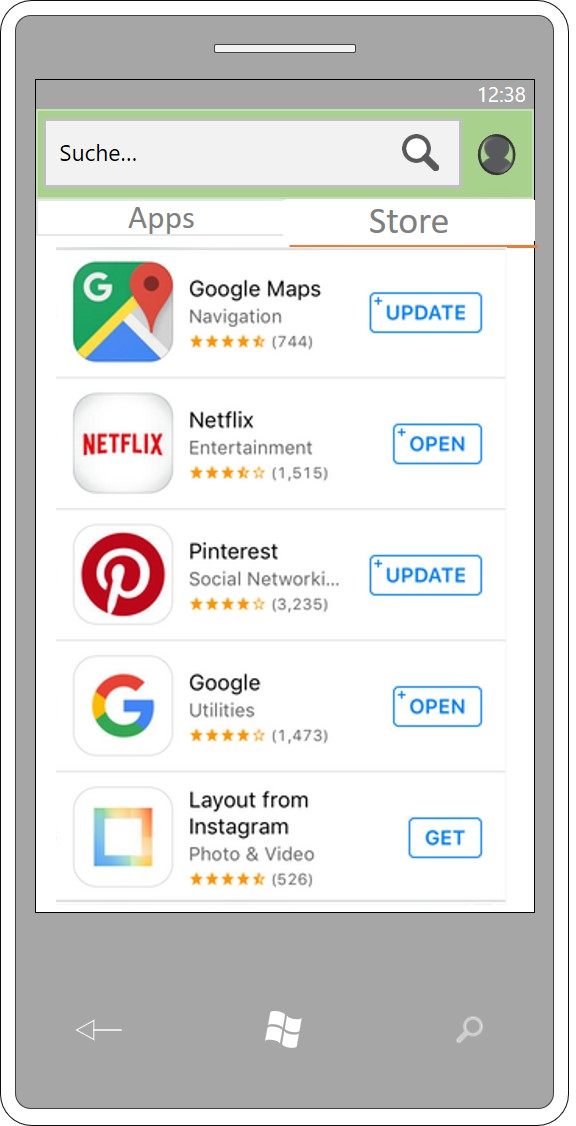
\includegraphics[width=1\linewidth]{Picture/App-Store}
		\caption{Store}
		\label{fig:prototyp1}
	\end{subfigure}%
	\begin{subfigure}{0.32\linewidth}
		\centering
		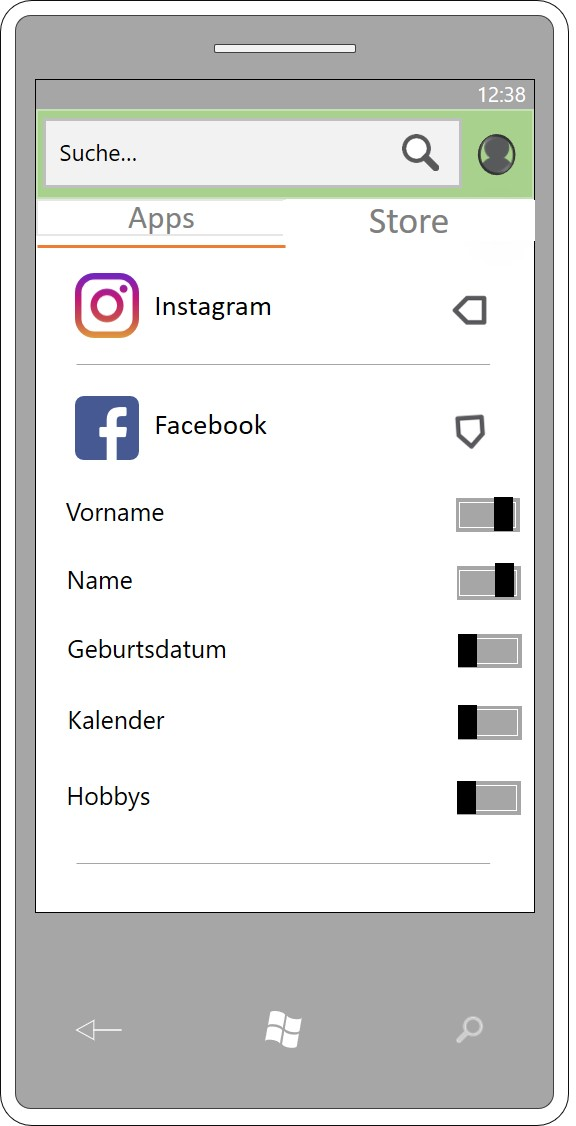
\includegraphics[width=1\linewidth]{Picture/App-Settings}
		\caption{Einstellungen}
		\label{fig:prototyp2}
	\end{subfigure}
	\begin{subfigure}{0.32\linewidth}
		\centering
		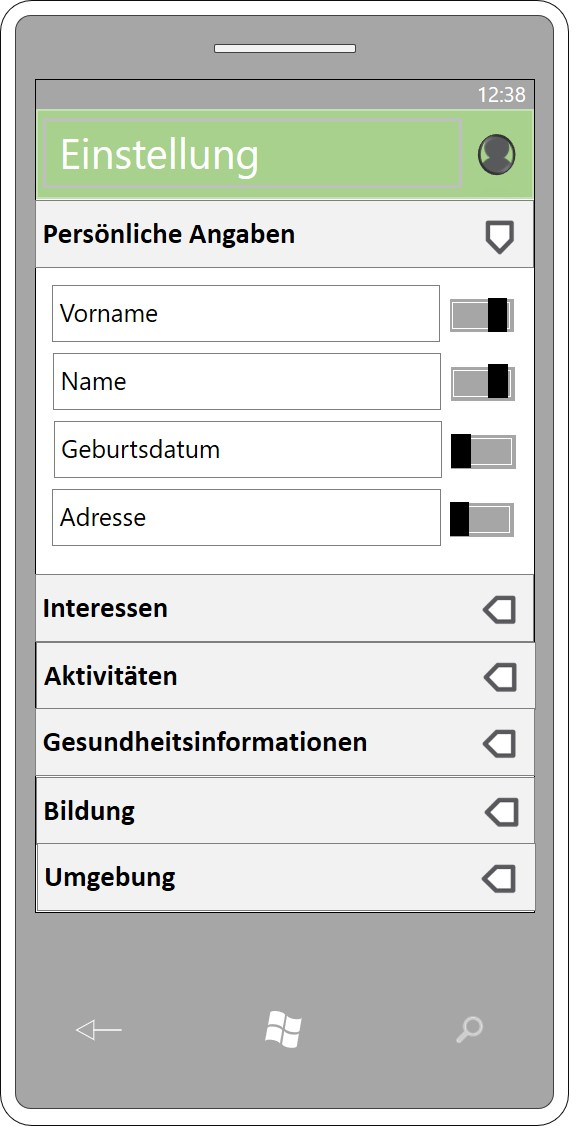
\includegraphics[width=1\linewidth]{Picture/App-Kontext}
		\caption{Nutzer Kontext}
		\label{fig:prototyp3}
	\end{subfigure}%
	\caption{Prototyp der App}
	\label{fig:prototyp}
\end{figure}











